\section{La page des tournois}

\begin{figure}[H]
\centering
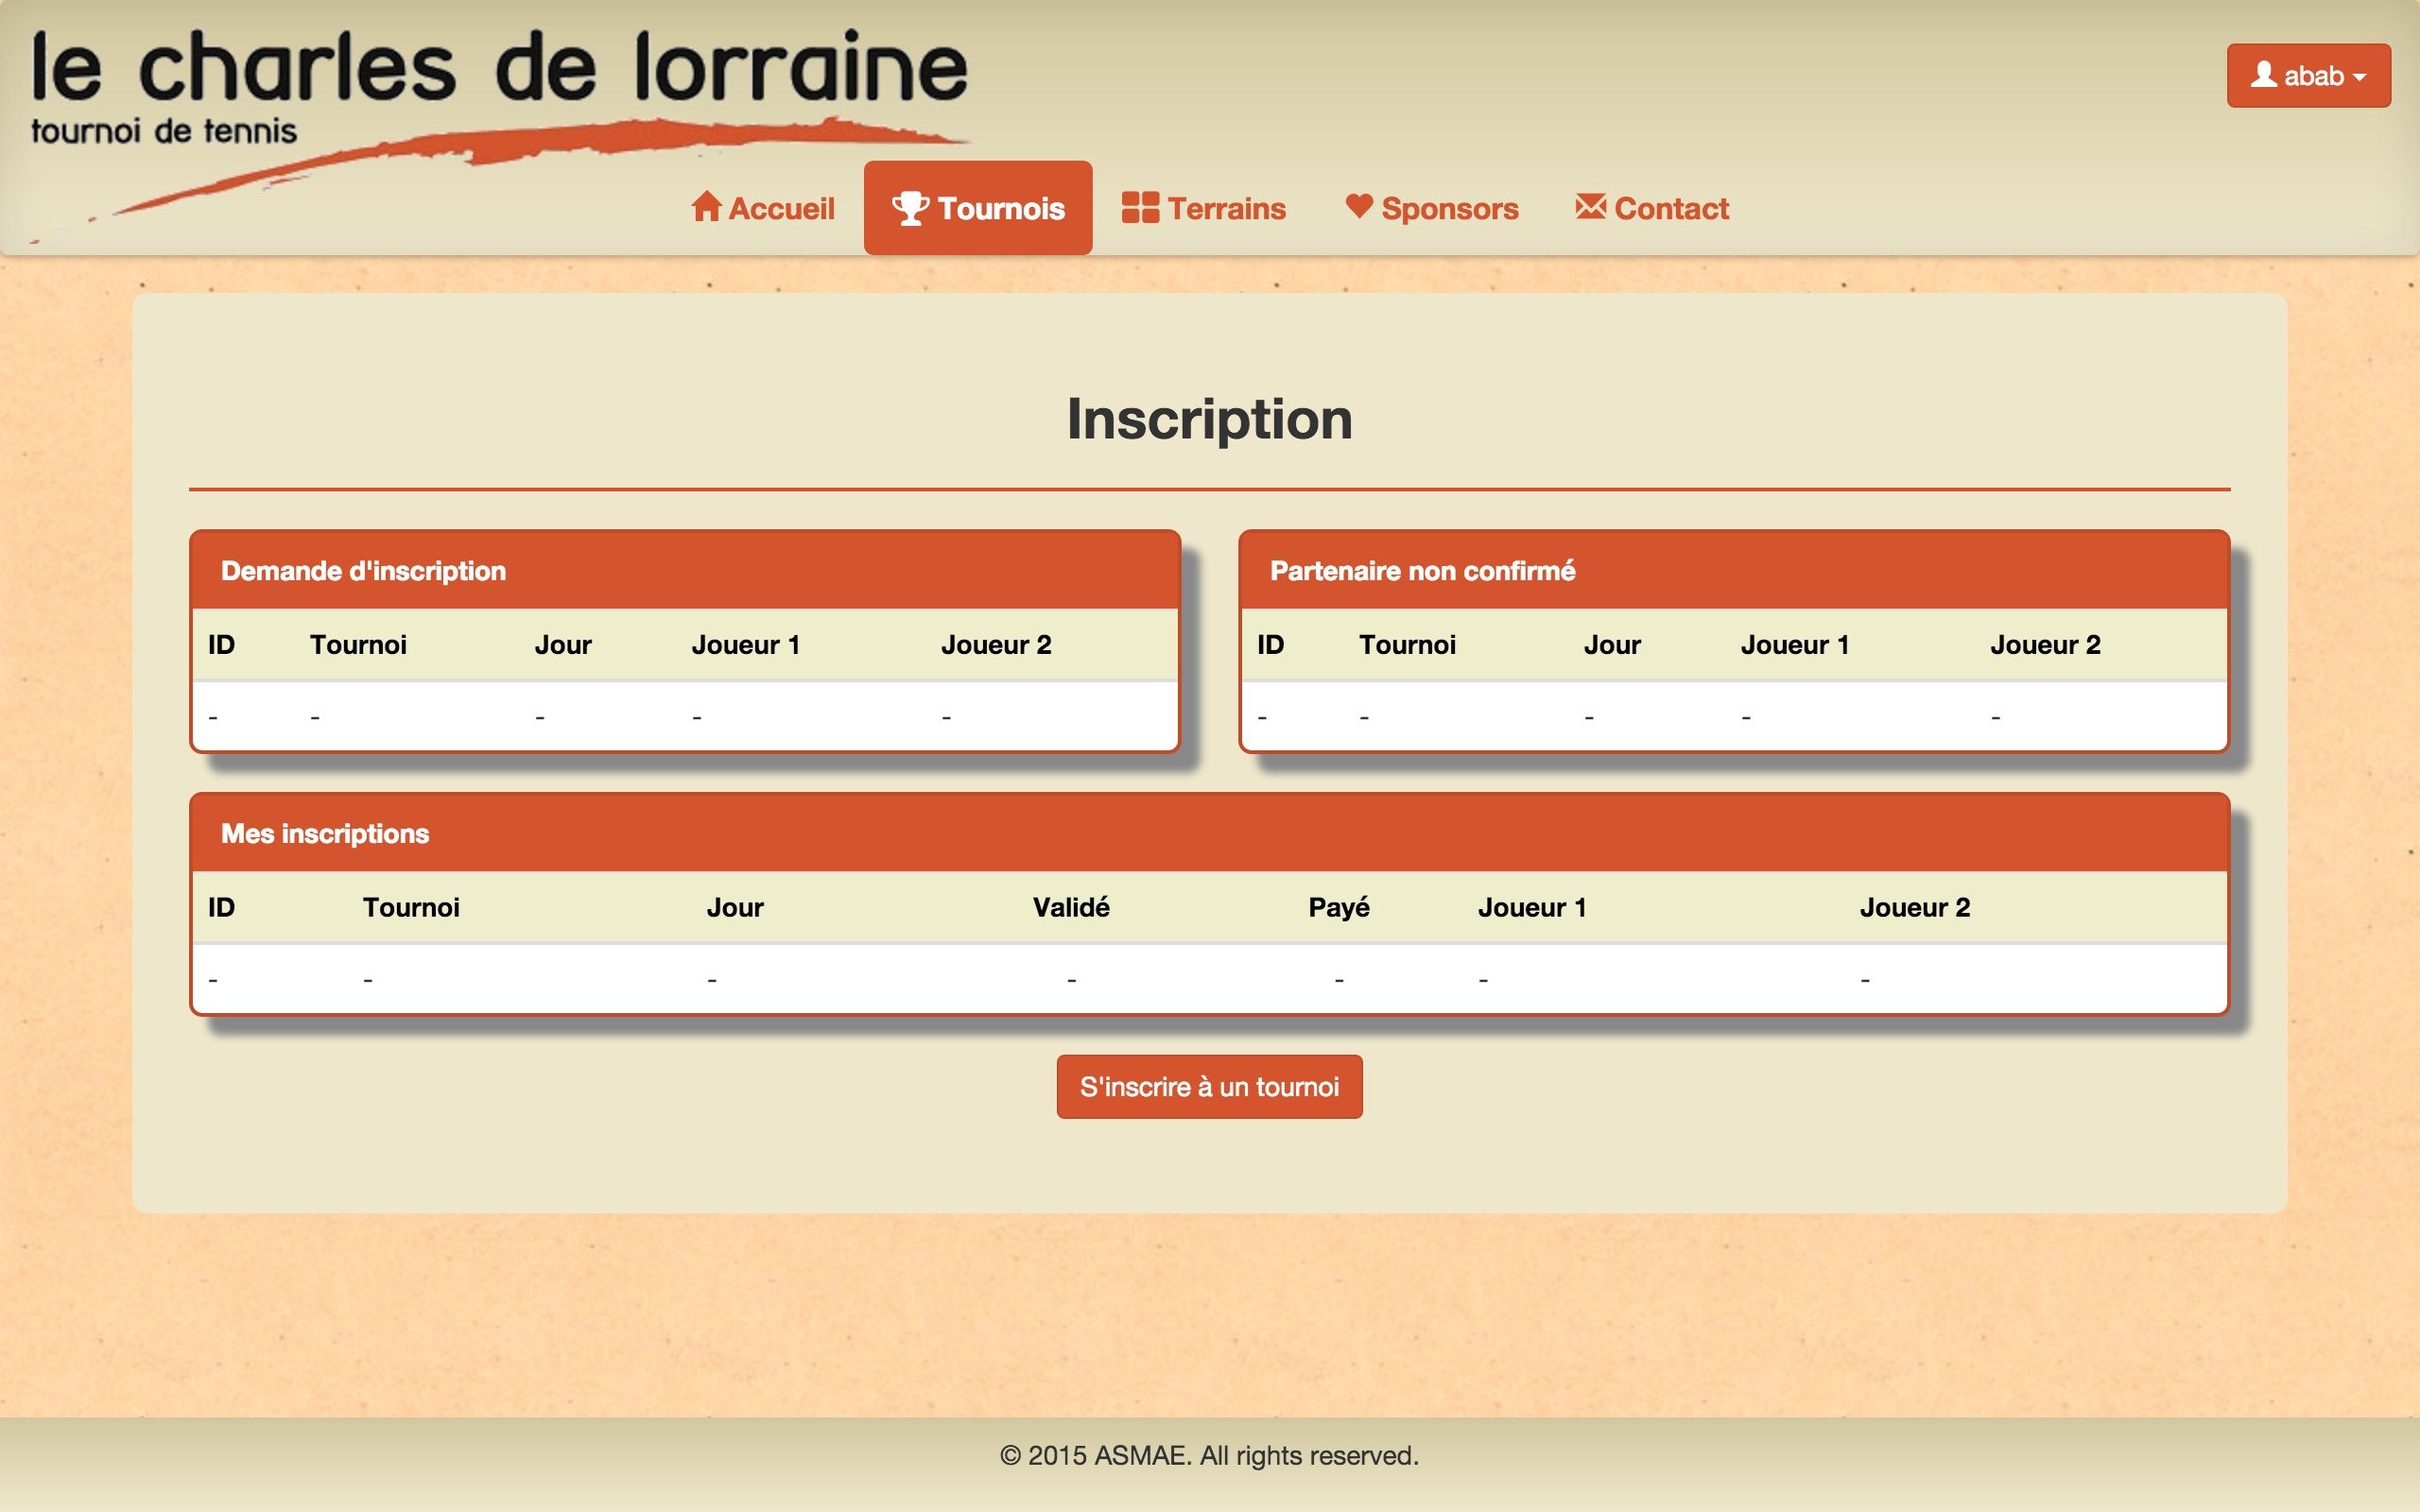
\includegraphics[scale=0.15]{page-tournois/page-tournois.jpg}
\caption{Page des tournois}
\end{figure}

Lorsque vous êtes connecté et aviez confimé l'adresse email de votre compte, vous pourrez accéder à la page \enquote{Tournois}.

\subsection{Vos inscriptions}

Depuis la page \enquote{Tournois}, vous pouvez gérer vos inscriptions. \newline

Il y a 3 catégories d'inscription : \newline

\begin{description}
    \item[Les demandes d'inscription] : elles émanent d'autres joueurs qui
    vous proposent de former une paire, vous pouvez cliquer dessus, faire vos
    choix et indiquer des commentaires supplémentaires pour l'équipe et ensuite
    valider ; ou vous pouvez refuser la demande du joueur.
    \item[Les partenaires non confirmés] : ce sont les demandes que vous avez
    faites à d'autres joueurs et qui sont en attente de confirmation de sa part.
    Si vous ne souhaitez plus proposer à l'autre joueur de former une paire,
    vous pouvez supprimer votre demande en cliquant dessus et en appuyant sur
    \textit{Supprimer}.
    \item[Les inscriptions confirmées] : elles signifient que vous et votre
    partenaire avez accepté de former une paire. Vous pouvez cliquer dessus
    pour voir un résumé de votre demande et effectuer votre paiement.
\end{description}

Lorsque le tournoi est en cours, vous pouvez consulter les activités du
tournoi, tout bas de la page \enquote{Tournois}.

\begin{figure}[H]
\centering
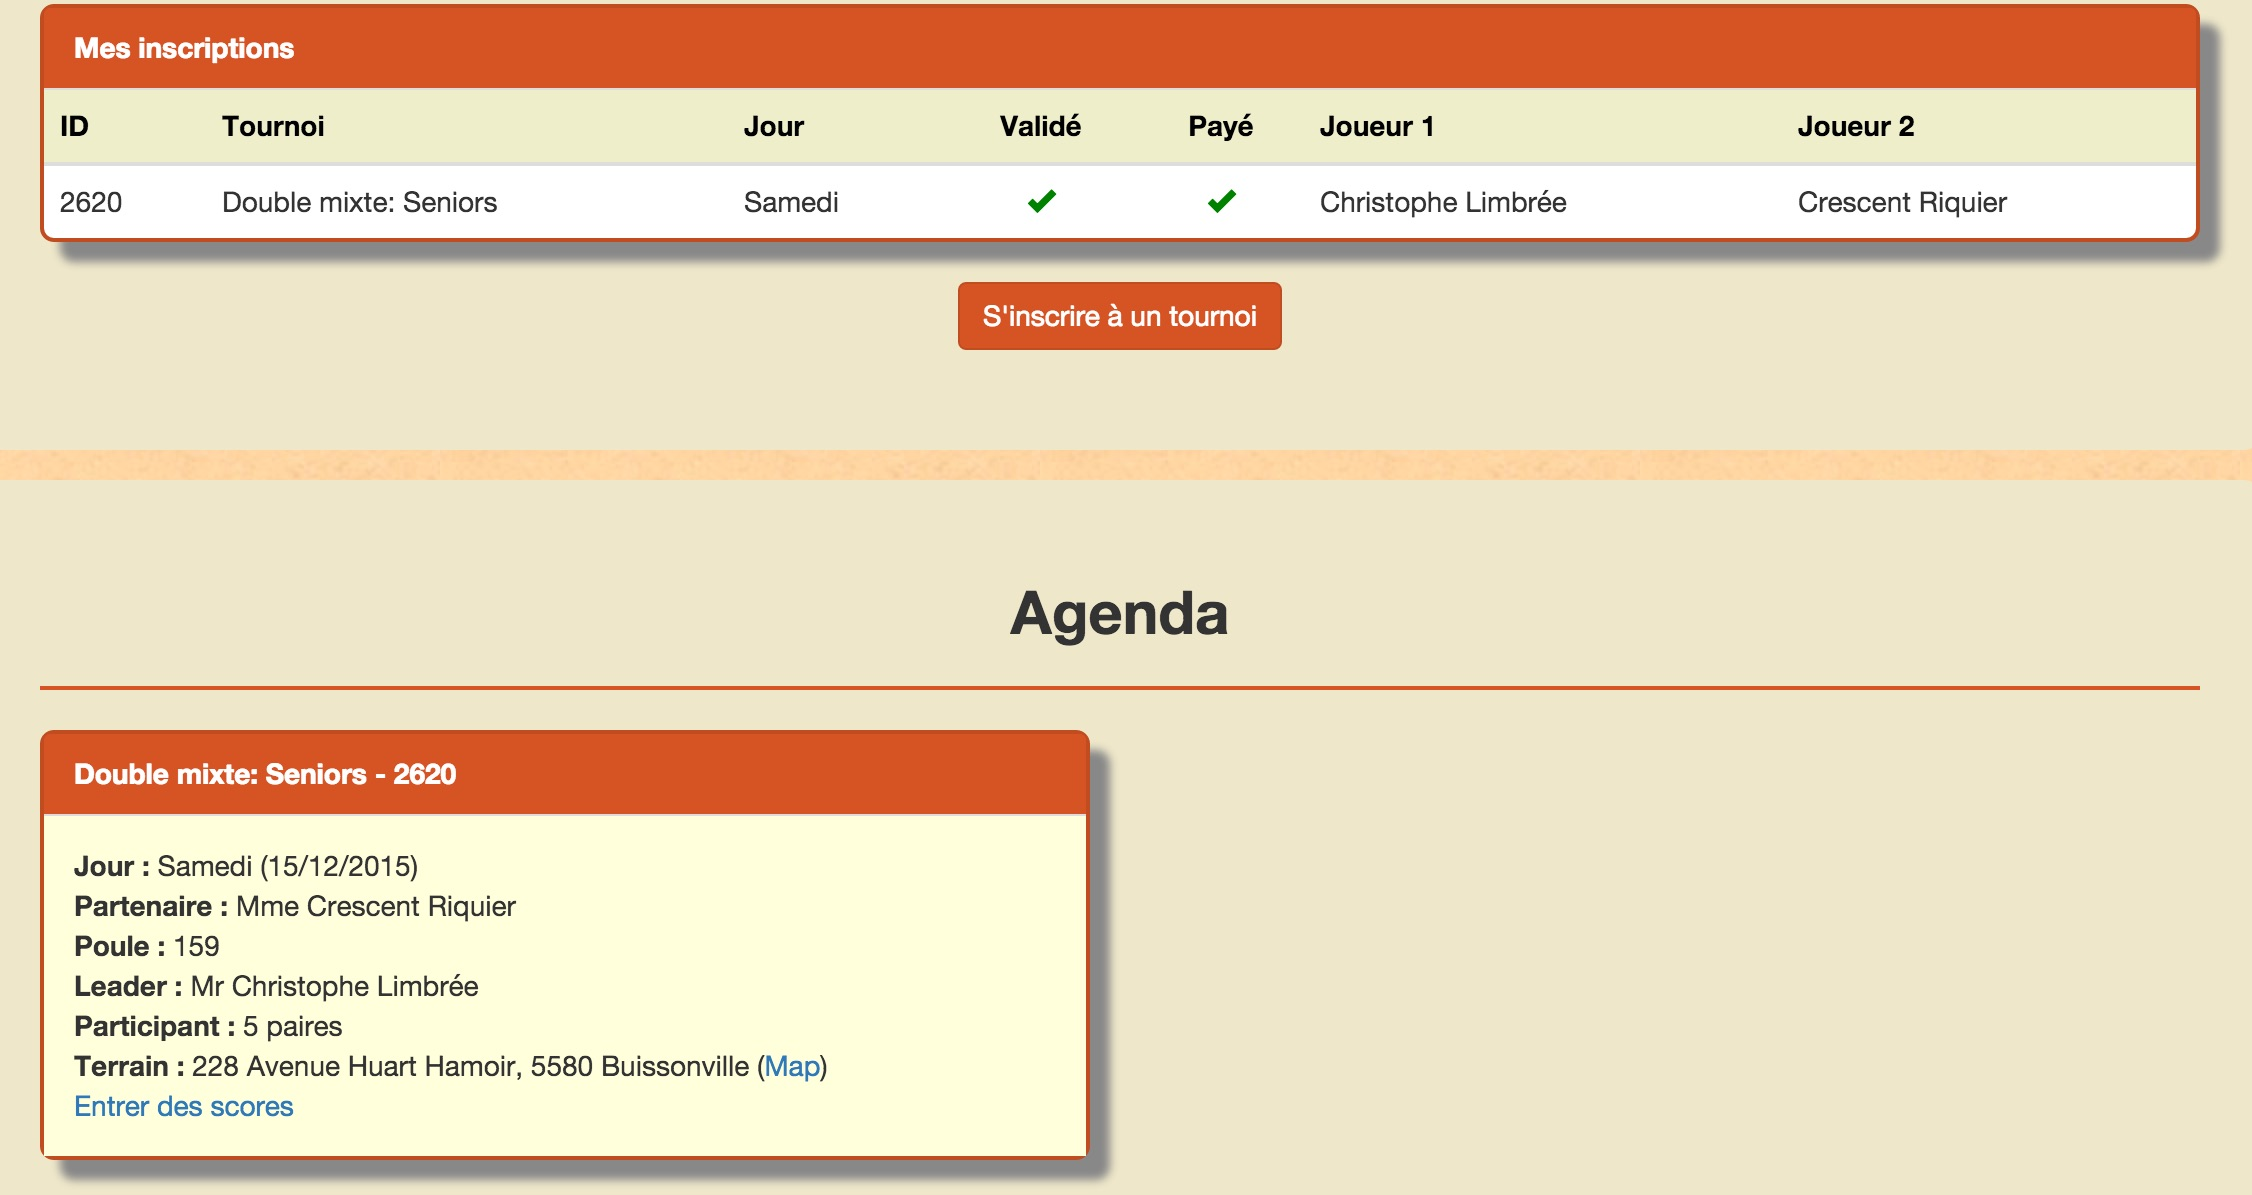
\includegraphics[scale=0.15]{page-tournois/page-tournois-agenda.jpg}
\caption{Page des tournois lorsque un tournoi est actif}
\end{figure}

Lorsque les poules du tournoi ont été créées, vous pouvez remplir les scores
des matchs de la poule dans laquelle vous participez. Notez cependant que
les scores entrées ne seront pas définitifs : un membre du staff verra ces
scores indiqués sur sa page de gestion des poules, mais elles ne seront
là qu'à dire indicatif. Les membres du staff ont toujours le dernier mot !

\begin{figure}[H]
\centering
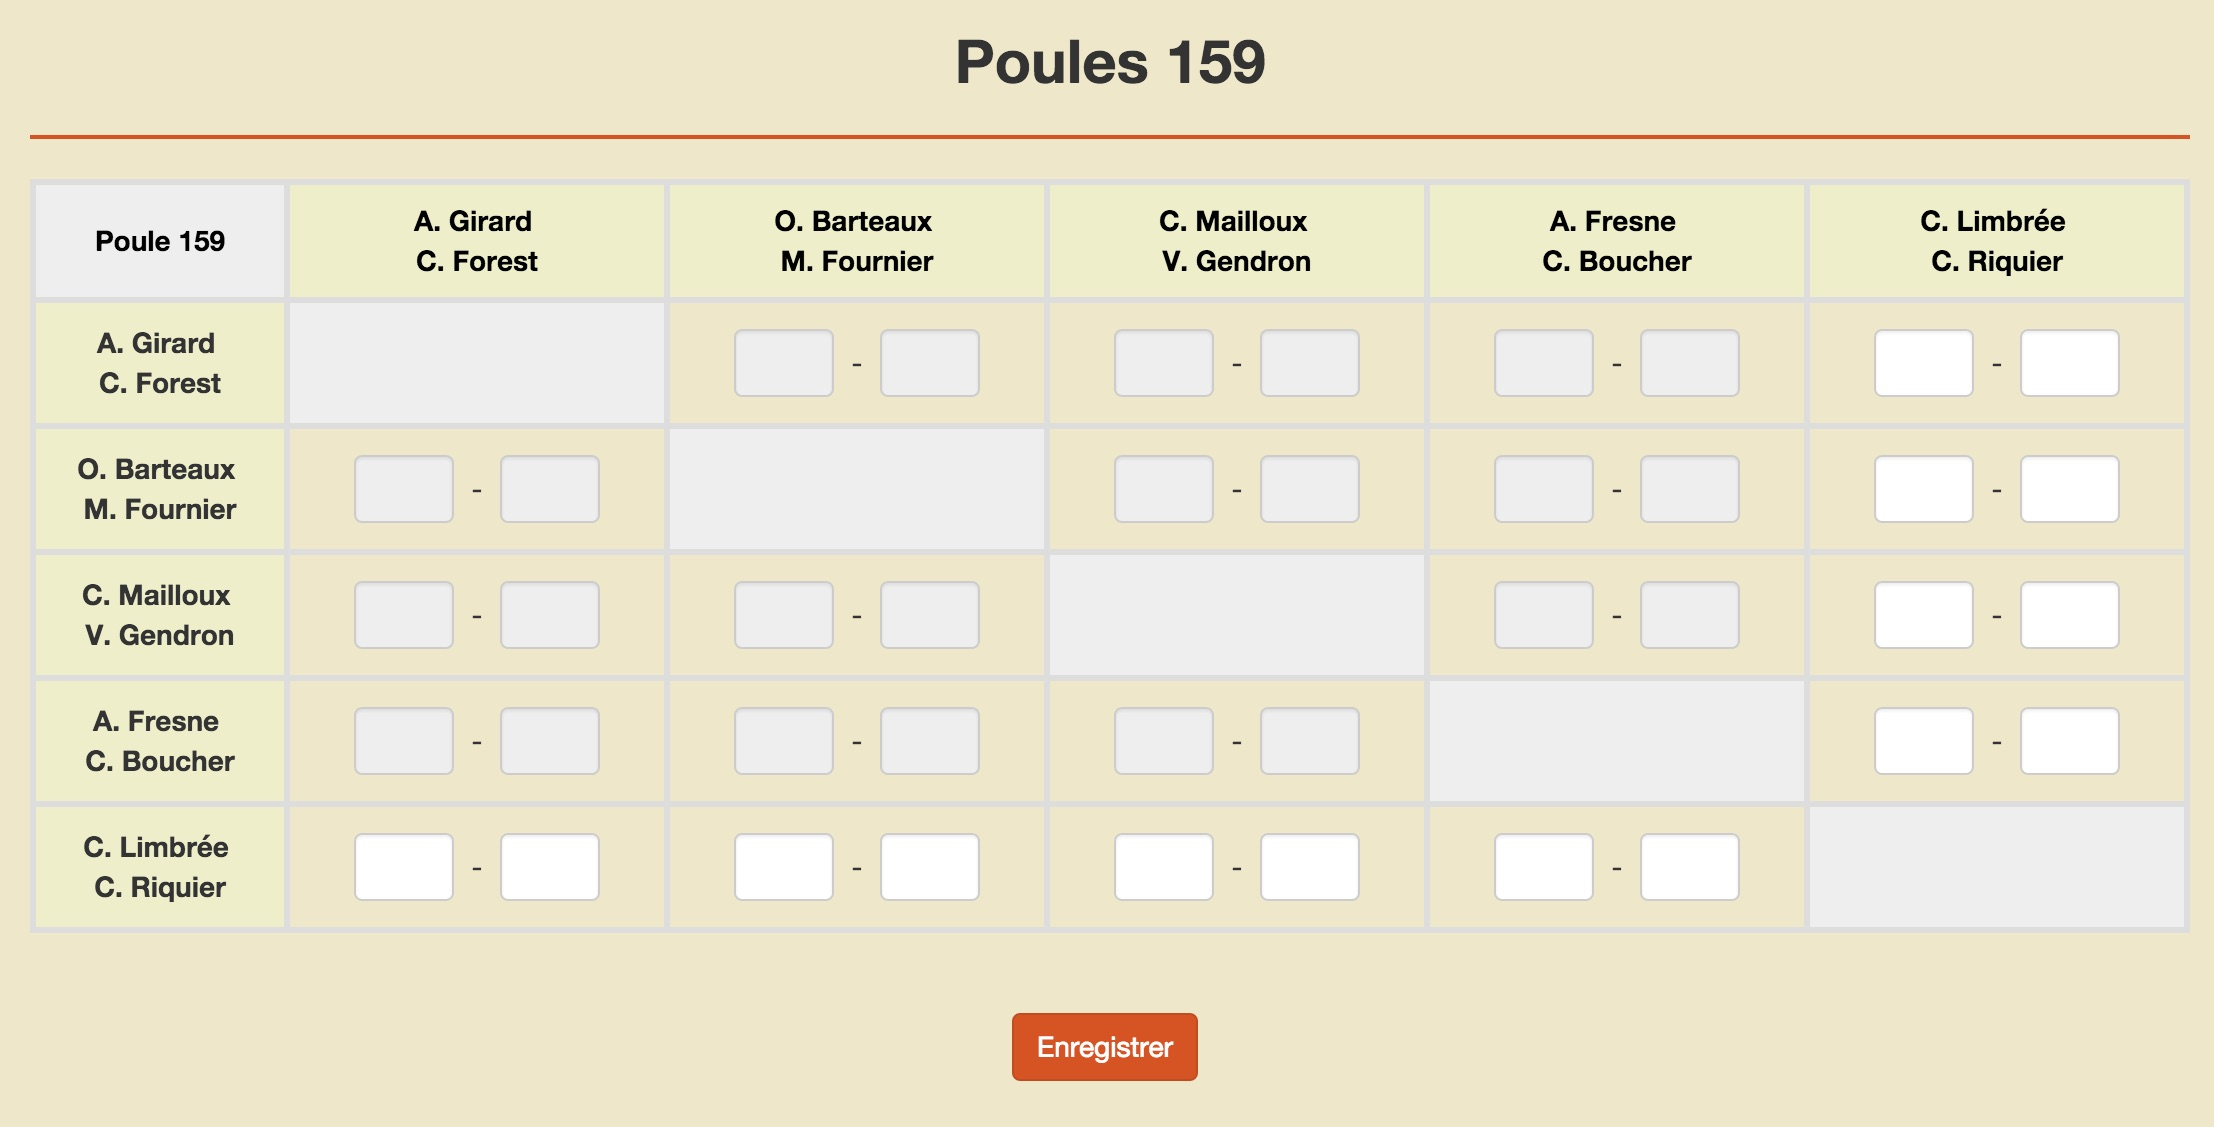
\includegraphics[scale=0.15]{page-tournois/page-tournois-scores.jpg}
\caption{Page de soumission des scores des matchs de la paire, du côté des joueurs}
\end{figure}